\subsection{Shape}

The shape of the robot was designed to convey friendliness, uniqueness, and a sense of purpose within its social environment. Taking inspiration from kitchen elements, the robot adopts a stylized form reminiscent of a cooking pot, reinforcing its role as a ticket dispenser for a microwave queue.

The overall geometry is conical, with a wide dodecagonal base that houses the movement module and narrows as it rises, creating a silhouette that is both functional and expressive. The lower section (in red) is where the wheels and internal electronics are stored. The transparency of the conical section allows for visual access to internal components and lighting, adding both a technological and playful aesthetic.

At the top of the robot, the head is formed by a metallic-looking circular cap with a symmetrical design, integrating visual sensors, lights, or interface points. A pair of stylized "ears" or "handles" give it a characterful appearance, reinforcing its role as a social entity that invites interaction. The shape also leaves space at the front for a clearly visible ticket dispensing area.

\begin{figure}[H]
    \centering
    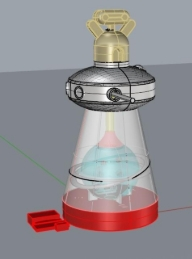
\includegraphics[width=0.6\linewidth]{../ReportMovementModule/images/Aspose.Words.728084da-df58-4b9d-a372-f65cffbdb23d.009.jpeg}
    \caption{Robot Shape Design}
\end{figure}
